\documentclass[11pt]{article}

\usepackage{amsmath}
\usepackage{amssymb}
\usepackage{subfigure}

\usepackage[font=footnotesize]{caption}
\usepackage{pgfplots}
\usepackage{tikz}

% Scriptsize axis style.
\pgfplotsset{every axis/.append style={tick label style={/pgf/number format/fixed},font=\scriptsize,ylabel near ticks,xlabel near ticks,grid=major}}

\begin{document}
\begin{figure}[t]
	\centering
	\subfigure[USPS]{
	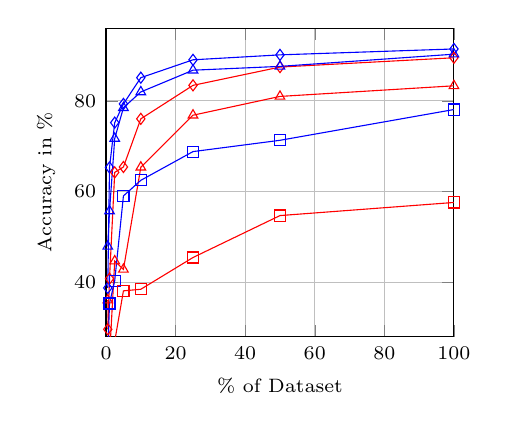
\begin{tikzpicture}
		\begin{axis}[%
			xlabel=\% of Dataset,
			ylabel=Accuracy in \%,
			height=5.5cm,
			width=6cm,
			ymax=96,
			ymin=28,
			xmin=0,
			xmax=100,
			%xmode=log,
            %log ticks with fixed point,
		]
        
        % T = 100
		\addplot[color=blue,mark=diamond] coordinates {
			(0.5,38.76)
			(1,65.32)
			(2.5,75.19)
			(5,79.32)
			(10,85.10)
			(25,89.04)
			(50,90.13)
			(100,91.43)
		};
		
		\addplot[color=red,mark=diamond] coordinates {
			(0.5,29.65)
			(1,40.81)
			(2.5,64.23)
			(5,65.42)
			(10,76.03)
			(25,83.41)
			(50,87.44)
			(100,89.49)
		};
		
		% T = 10
		\addplot[color=blue,mark=triangle] coordinates {
			(0.5,47.93)
			(1,55.71)
			(2.5,71.70)
			(5,78.48)
			(10,81.96)
			(25,86.75)
			(50,87.59)
			(100,90.28)
		};
		
		\addplot[color=red,mark=triangle] coordinates {
			(0.5,36.07)
			(1,23.47)
			(2.5,44.69)
			(5,42.85)
			(10,65.37)
			(25,76.83)
			(50,80.97)
			(100,83.31)
		};
		
		% T = 1
		\addplot[color=blue,mark=square] coordinates {
			(0.5,24.36)
			(1,35.33)
			(2.5,40.36)
			(5,59.04)
			(10,62.48)
			(25,68.81)
			(50,71.30)
			(100,78.08)
		};
		
		\addplot[color=red,mark=square] coordinates {
			(0.5,17.89)
			(1,23.47)
			(2.5,27.01)
			(5,38.12)
			(10,38.47)
			(25,45.47)
			(50,54.71)
			(100,57.60)
		};
		\end{axis}
	\end{tikzpicture}
	}
	\subfigure[MNIST]{
	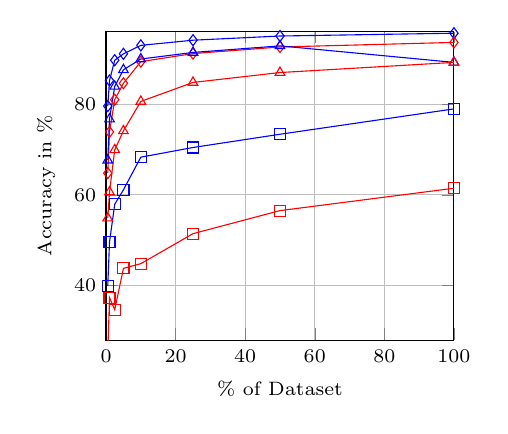
\begin{tikzpicture}
		\begin{axis}[%
			xlabel=\% of Dataset,
			ylabel=Accuracy in \%,
			height=5.5cm,
			width=6cm,
			ymax=96,
			ymin=28,
			xmin=0,
			xmax=100,
			%xmode=log,
            %log ticks with fixed point,
		]

        % T = 100
		\addplot[color=blue,mark=diamond] coordinates {
			(0.5,79.58)
			(1,85.22)
			(2.5,89.69)
			(5,91.09)
			(10,92.96)
			(25,94.10)
			(50,95.02)
			(100,95.64)
		};
		\label{plot:mnist-100-offline}
		
		\addplot[color=red,mark=diamond] coordinates {
			(0.5,64.80)
			(1,73.88)
			(2.5,80.98)
			(5,84.61)
			(10,89.37)
			(25,91.15)
			(50,92.60)
			(100,93.61)
		};
		\label{plot:mnist-100-online}
		
		% t = 10
		\addplot[color=blue,mark=triangle] coordinates {
			(0.5,67.65)
			(1,76.72)
			(2.5,83.91)
			(5,87.57)
			(10,89.95)
			(25,91.40)
			(50,92.85)
			(100,89.21)
		};
		\label{plot:mnist-10-offline}
		
		\addplot[color=red,mark=triangle] coordinates {
			(0.5,54.90)
			(1,60.64)
			(2.5,69.93)
			(5,74.11)
			(10,80.60)
			(25,84.79)
			(50,86.97)
			(100,89.21)
		};
		\label{plot:mnist-10-online}
		
		% T = 1
		\addplot[color=blue,mark=square] coordinates {
			(0.5,39.98)
			(1,49.64)
			(2.5,57.94)
			(5,61.12)
			(10,68.32)
			(25,70.45)
			(50,73.37)
			(100,78.96)
		};
		\label{plot:mnist-1-offline}
		
		\addplot[color=red,mark=square] coordinates {
			(0.5,25.15)
			(1,37.37)
			(2.5,34.70)
			(5,43.81)
			(10,44.85)
			(25,51.46)
			(50,56.54)
			(100,61.47)
		};
		\label{plot:mnist-1-online}
		\end{axis}
	\end{tikzpicture}
	}
	\caption{Comparison of on-line and off-line Random Forests on the USPS \cite{Hull} and MNIST \cite{LeCunBottouBengioHaffner} datasets. Note that the MNIST dataset provides $60,000$ training examples and $10,000$ test examples with dimension $28 \times 28$., while the USPS dataset only provides $7,291$ training examples and $2,007$ test examples with dimension $16 \times 16$. Experiments where conducted for different forest sizes $T$: \ref{plot:mnist-1-offline}, \ref{plot:mnist-1-online} $T = 1$; \ref{plot:mnist-10-offline}, \ref{plot:mnist-10-online} $T = 10$; and \ref{plot:mnist-100-offline}, \ref{plot:mnist-100-online} $T = 100$}
	\label{fig:online-random-forests-experiments}
\end{figure}

\begin{thebibliography}{1}
	 \bibitem{Hull}
	 J. J. Hull,
	 \emph{A Database for Handwritten Text Recognition Research},
	 Transactions on Pattern Analysis and Machine Intelligence,
	 1994.
	 
	 \bibitem{LeCunBottouBengioHaffner}
	 Y. LeCun,
	 L. Bottou,
	 Y. Bengio,
	 P. Haffner,
	 \emph{Gradient-Based Learning Applied to Document Recognition},
	 Proceedings of the IEEE,
	 1998.
\end{thebibliography}
\end{document}
